\documentclass[a4paper,12pt]{article}

\usepackage[utf8]{inputenc}
\usepackage[portuguese]{babel}
\usepackage{graphicx}

\title{Relatório\\[1.5em]
Laboratórios de Informática I\\
\emph{LightBot em Haskell}}

\author{Paulo Franco, A75871 - Nuno Armada, A75877}

\date{2014/2015}

\begin{document}

\maketitle
\clearpage
\tableofcontents

\clearpage
\section{Introdução}

\paragraph{}
O presente relatório vai abordar os aspetos mais importantes das diferentes tarefas levadas a cabo para recriar o jogo bastante conhecido, \emph{Lighbot}. Para tal, desenvolvemos um algoritmo utilizando a linguagem de programação funcional \emph{Haskell}.
\paragraph{}
O projeto foi dividido em duas fases, com as tarefas A, B e C na primeira, e D e E na segunda fase.


\begin{figure}[h]
\centering

\includegraphics[scale=0.5]{./imagens/logo.jpg}
\caption{Logotipo do jogo \emph{Lightbot}} \label{Fig:Logo}
\end{figure}


\section{Tarefa A}

\paragraph{}
A tarefa A tem como objetivo testar se um tabuleiro de jogo é válido.
O programa deve ler do \emph{stdin} um ficheiro de texto e verificar se segue a especificação apresentada no enunciado. Como resultado, o programa deve imprimir no \emph{stdout} uma única linha contendo:
\begin{itemize}
\item \textbf{OK}, se o ficheiro estiver conforme a especificação;
\item \textbf{num}, no caso de erro (sendo num o número da linha onde ocorre o primeiro erro).

\end{itemize}

\subsection{Problema vs. Algoritmo}

\paragraph{}
Resolvemos, antes de pensar em código \emph{Haskell}, estruturar todo o problema proposto com uma caneta e algum papel. Definimos as funções básicas que eram necessárias e o caminho que íamos adotar para chegar à solução final. Posto isso, passamos para o código.

\paragraph{}
Em primeiro lugar, separamos em 3 variáveis distintas as 3 componentes que precisávamos de avaliar do \emph{input} que nos era fornecido: tabuleiro, coordenadas e comandos.
Logo de seguida, criamos uma função para verificar a validade de cada uma destas componentes. Atribuímos esses resultados a novas variáveis. No final, no caso de erros, apresentamos o número da linha onde é encontrado o primeiro erro. No caso de o tabuleiro ser válido, apresentamos "OK".



\subsection{Testes da tarefa A}

\paragraph{}
Criámos diversos tabuleiros com diferentes objetivos de teste, dos quais:
\begin{itemize}
\item Tabuleiro

Testar se o tabuleiro era somente constituído por letras maiúsculas e/ou minúsculas.
\item Coordenadas

Testar se as coordenadas estavam no formato correto.
\item Comandos

Testar se a linha de comandos estão no formato correto, isto é, somente com os carateres maiúsculos LSAED
\item Outros aspetos

Verificar se depois da linha dos comandos não existem mais carateres

\end{itemize}

\section{Tarefa B}

\paragraph{}
A tarefa B tem como objetivo executar o primeiro comando para um tabuleiro válido.
\paragraph{}
O programa deve ler do \emph{stdin} um ficheiro de texto com a descrição do tabuleiro; o estado inicial do \emph{Robot}; e a sequência de comandos (conforme formato especificado no enunciado). Deve assumir que o formato dos dados de entrada é válido. Como resultado, o programa deve imprimir no \emph{stdout}:
\begin{itemize}
\item \textbf{ERRO}, se o primeiro comando não for aplicável (e.g. tentar executar o comando L sobre uma posição sem lâmpada);

\item \textbf{xcoord ycoord orient}, no caso de o comando ser aplicável (onde \emph{xcoord, ycoord} e \emph{orient} denotam respetivamente as coordenadas x e y do \emph{Robot}, e orient a sua orientação.
\end{itemize}

\subsection{Resolução do problema}

\paragraph{}
Já mais à vontade com a linguagem \emph{Haskell}, nesta tarefa o procedimento de pensar no problema e transformá-lo em \emph{Haskell} foi mais simples. Começamos por definir tipos para que fosse mais fácil a leitura do código. Mantivemos as variáveis que separavam as 3 componentes distintas provenientes do \emph{stdin}, e criamos algumas outras: tamTab, que guarda num tipo (Int,Int) o tamanho xx yy do tabuleiro; pInicial que guarda a posição inicial do \emph{Robot}, num formato (Int,Int,Char).
\paragraph{}
Criámos uma função para executar um comando, assumindo que deveria cumprir todas as regras impostas pelo jogo. Essa função retorna a posição do robot após executar o comando. Se essa posição for válida, isto é, se o comando for aplicado com sucesso, irá devolver essa mesma posição. Caso contrário, irá devolver a mensagem ERRO.


\subsection{Testes da tarefa B}
Criámos diversos tabuleiros com diferentes objetivos de teste:

\begin{itemize}

\item {\textbf{A}} - Andar

Avança uma posição se não estiver num dos limites e se o destino estiver no mesmo nível.

\item {\textbf{S}} - Saltar

Neste caso, permitimos que o \emph{Robot} suba para o nível imediatamente a seguir ou desça para qualquer nível

\item {\textbf{E}} - Esquerda ou {\textbf{D}} - Direita

Este comando faz com que o \emph{Robot} rode para a esquerda ou direita, trocando assim a orientação

\item {\textbf{L}} - Lâmpada

Acende ou apaga a lâmpada, se essa existir na atual posição do \emph{Robot}

\end{itemize}

\section{Tarefa C}

\paragraph{}
O programa deve executar a sequência de comandos no \emph{Robot}. Deve atender aos seguintes aspetos:

\begin{itemize}

\item Assume-se que o formato do ficheiro de entrada é válido.

\item Os comandos são executados em sequência.

\item Comandos que não sejam aplicáveis deverão deixar o estado do \emph{robot} inalterado (tal como na versão do jogo online).

\item Sempre que um comando L for executado com sucesso, deverá ser impressa uma linha contendo as coordenadas x e y da posição onde o \emph{robot} se encontra (separadas por um único espaço).

\item Quando todas a lâmpadas do tabuleiro se encontrarem ligadas, o programa imprime uma linha com a mensagem FIM (\emph{tickcount}) (em que (\emph{tickcount}) é o número de comandos válidos executados);

\item Se a sequência de comandos terminar sem que todas as lâmpadas se encontrem ligadas deve imprimir a mensagem INCOMPLETO.

\end{itemize}

\subsection{Execução do jogo}

\paragraph{}
A tarefa C foi talvez a mais fácil de todas. Na verdade só teríamos de criar uma recursividade para a tarefa B. Foi mais ou menos o que aconteceu.

\paragraph{}
Criámos uma nova variável para guardar o número de lâmpadas que cada tabuleiro continha. De seguida, criámos uma função para executar todos os comandos fornecido pelo \emph{stdin}, em sequência.

\subsection{Testes da tarefa C}
Criámos diversos tabuleiros com diferentes objetivos de teste:

\begin{itemize}
\item {\textbf{L - Lâmpada}}

Acende ou apaga a lâmpada, se existir na atual posição do \emph{Robot}. Se tentar acender uma lâmpada que já se encontra acesa, então este vai apagá-la. Irá imprimir a coordenada sempre que o comando L for válido.

\item {\textbf{Número lâmpadas acesas}}

Executa a lista de comandos até que o número de lâmpadas acesa seja igual ao número de lâmpadas do tabuleiro. Se acabar a lista de comandos e essa condição não se verificar, devolve "INCOMPLETO", caso contrario, devolve "FIM k" em que k é o número de comandos válidos executados.

\item {\textbf{Comandos inválidos}}

Se um comando for inválido, este vai-se manter na mesma posição e vai tentar efetuar o comando seguinte.

\end{itemize}


\section{Tarefa D}

\paragraph{}
A tarefa D tem como objetivo imprimir numa linha o \emph{stdout} com os comandos necessários para resolver um tabuleiro lido do \emph{stdin}, partindo da posição inicial e acendendo todas as lâmpadas disponíveis.

\paragraph{}
Numa primeira fase, tal como indicado no enunciado, começamos por pensar em solucionar um tabuleiro simples, ou seja, seria sempre possível movimentar o \emph{robot} para qualquer posição válida do tabuleiro. A diferença do nível entre as posições nunca seria superior a 1. Numa segunda fase, avançamos para os tabuleiros complexos, onde nem todas as movimentações eram possíveis e podia existir um único caminho possível para uma determinada lâmpada.

\subsection{O Algoritmo}

\paragraph{}
Antes de iniciar, foram alguns os dias a pensar na melhor forma de abordar este problema. Temos consciência que poderá ser um problema complexo se pensado até ao ínfimo pormenor. No entanto, numa primeira fase pensamos nos dados básicos que iríamos precisar para manipular e chegar a uma solução, dos quais destacamos: coordenada exata das lâmpadas; quais as lâmpadas mais próximas a partir de uma determinada posição. Com isto, sempre que se movimentasse saberia sempre quais as lâmpadas mais próximas da posição em que o \emph{robot} se encontrava.
Bastaria então, seguir as direções para todas as lâmpadas até que todas estivessem acesas. Para um tabuleiro simples, isto seria suficiente. E foi.

\paragraph{}
Quando já conseguíamos resolver qualquer tabuleiro simples, passamos então para os tabuleiros complexos. Sabíamos que agora não seria tão fácil chegar a uma boa solução. Pensamos então no seguinte: E se fizermos, de forma exaustiva, diversas tentativas até encontrarmos a lâmpada pretendida?! Assim foi. Antes de tudo seria preciso saber, numa determinada posição, quais as movimentações possíveis. Tendo isso, só teria que ir tentando todas elas até chegar à lâmpada. Caso chegasse a um caminho sem saída e esse fosse diferente da posição da lâmpada, começaria do inicio e adicionaria aquela mesma posição a uma lista de caminhos sem saída para não voltar a passar por lá. Importante referir que teria que guardar também o caminho percorrido para não o repetir e cair no erro de ficar às voltas.

Era uma forma que não seria a mais eficiente, mas foi a primeira ideia de resolução. Bastou pôr em prática, e conseguimos assim resolver grande parte dos tabuleiros.

\subsection{Tabuleiros simples}

\paragraph{}

Começamos por fazer uma função que determinava, a partir de um tabuleiro, quais as coordenadas das lâmpadas. Logo de seguida, fizemos a função que determina qual a distância entre a posição em que o \emph{robot} se encontra até todas as lâmpadas que ainda se encontram por acender. Subtraímos a coordenada da lâmpada pela posição do \emph{robot} e isso diz-nos quais as direções para aquela lâmpada. No final, foi só ordenar o resultado pela condição (x+y), pois representaria o número de andamentos que teriamos que fazer até chegar àquela lâmpada.

\paragraph{}
Posto isto, só faltava fazer a função para resolver o problema. Criámos uma função para ler a lista das lâmpadas mais próximas e fazer andamentos sempre em direção à primeira coordenada dessa lista, até que esse lista ficasse vazia (momento em que todas as lâmpadas estariam acesas), resolvendo o tabuleiro de uma forma lógica e expedita.

\subsection{Tabuleiros complexos}

\paragraph{}
Nesta fase, começamos por criar uma função que permitia saber, numa determinada posição, quais as movimentações possíveis. De seguida, uma função que devolvia os comandos necessários para chegar a uma dessas movimentações.
\paragraph{}
Agora faltava a função que testava exaustivamente todos os caminhos até chegar a uma determinada lâmpada. No final, apenas teríamos que fazer a recursividade para acender todas as lâmpadas do tabuleiro.

\paragraph{}
Foi necessário criar uma forma de verificar os caminhos possíveis e marcar os caminhos já percorridos, guardando-os numa lista, para que só voltassem a ser testados na falta de outras alternativas. Como é demonstrado na tabela seguinte, o único caminho possível é o que está destacado, a \emph{\textbf{bold}}, portanto tínhamos que evitar repetir testar todas as outras posições mais do que uma vez. Sempre que voltávamos à posição inicial, por não ser possível chegar à lâmpada com o percurso anterior, adicionamos essa posição a uma lista. Assim, de cada vez que o \emph{robot} saltava para o interior do tabuleiro, na próxima tentativa já iria ficar mais próximo da lâmpada.



\begin{table}[h]
\centering
\begin{tabular}{|c|c|c|c|c|c|c|}
\hline
\textbf{5} & \textbf{E} & \textbf{f} & \textbf{g} & \textbf{f} & \textbf{g} & \textbf{f} \\ \hline
\textbf{4} & a & b & b & b & b & \textbf{g} \\ \hline
\textbf{3} & b & c & c & e & b & \textbf{f} \\ \hline
\textbf{2} & c & c & c & e & b & \textbf{g} \\ \hline
\textbf{1} & b & b & b & b & b & \textbf{f} \\ \hline
\textbf{0} & \textbf{a} & \textbf{b} & \textbf{c} & \textbf{d} & \textbf{e} & \textbf{e} \\ \hline
\textbf{Y/X} & \textbf{0} & \textbf{1} & \textbf{2} & \textbf{3} & \textbf{4} & \textbf{5} \\ \hline
\end{tabular}
\caption{Caso de um tabuleiro com um único percurso possível} \label{Tab:Exemplo}
\end{table}

\paragraph{}

Posteriormente, tivemos que pensar na forma como o \emph{robot} se iria movimentar, que lâmpada iria escolher primeiro, e depois e depois. Achamos então que, se seguíssemos o mesmo modelo dos tabuleiros simples conseguiríamos otimizar o percurso do \emph{robot}. Usamos também as lâmpadas mais próximas, recalculando sempre que chegávamos à lâmpada que queiramos acender. Uma a uma, até acendermos todas as lâmpadas do tabuleiro.
\paragraph{}
Tudo funcionou conforme prevíamos, mas os resultados dos comandos gerados ainda eram muito extensos. Observamos que o \emph{robot} estava a passar por cima de algumas lâmpadas durante o seu percurso para apagar uma determinada lâmpada, e não as apagava. Alteramos essa situação e ficamos assim com um resultado bem mais apresentável e eficaz.
\paragraph{}
Faltava ainda verificar uma das hipóteses que tínhamos previsto na fase inicial deste tipo de tabuleiros: o caso de termos uma lâmpada num "buraco". Sabíamos que este teria que ser a última a ser resolvida. Arranjamos então uma forma de prever isso, não totalmente eficaz pois encontramos algumas falhas, mas deixa essa lâmpada para ultimo no caso da mesma se encontrar numa posição em que, depois de lá chegar, não permitisse mais movimentações.

\paragraph{}
Como já tínhamos 18 pontos no \emph{mooshak} e o tempo disponível para despender neste trabalho não era muito, fruto da vida profissional de cada membro do grupo, decidimos passar à próxima tarefa pois parecia também bastante aliciante.


\subsection{Testes da tarefa D}

\paragraph{}
Os tabuleiros criados para testar esta tarefa são de quatro tipos:
\begin{itemize}
\item Simples

Tabuleiros em que é sempre possível saltar ou avançar para qualquer posição válida do tabuleiro e uma lâmpada, mas a iniciarem em diferentes locais e/ou orientações.
\item Simples com várias lâmpadas

Tabuleiro em que é sempre possível saltar ou avançar para qualquer posição válida do tabuleiro mas com várias lâmpadas, destinados a perceber melhores formas de analisar o problema.
\item Complexos

Com estes tabuleiros pretendemos aprimorar o algoritmo de forma a minimizar o Nº de comandos para solucionar problemas mais complexos.


\end{itemize}
\section{Tarefa E}

\paragraph{}
Apesar de no enunciado referir que o input fornecido era igual ao da primeira fase do projeto, decidimos abranger outra situação que para nós pareceu de alguma forma lógica: se na tarefa D estivermos a gerar comandos para um tabuleiro, agora vamos dar animação a esse resultado. A nossa tarefa E usa os comandos fornecidos pelo \emph{input} se estes estiverem presentes, caso contrário, lê o tabuleiro e posição inicial, resolve o tabuleiro e cria a animação com os comandos gerados.

No caso dos comandos gerados nunca vamos ter situações em que o \emph{robot} acende e volta a apagar uma lâmpada, mas no caso dos comandos fornecidos apresentarem essa situação, tivemos também atenção a isso, voltando assim a apagar/acender a lâmpada sempre que o comando L fôr usado naquela posição.

É descrito ao lado do tabuleiro se os comandos foram \emph{Comandos Lidos:} ou \emph{Comandos Gerados:}
\paragraph{}
Nenhum dos dois conhecia \emph{X3dom}, mas achamos desde o início que era algo que íamos gostar de construir. Decidimos dar um pouco mais de nós nesta tarefa.

\subsection{Criação da estrutura da página/\emph{X3Dom}}

\paragraph{}
Depois de uma fase para perceber como criar objetos e respetivas animações, começamos a desenvolver aquilo que seria o nosso \emph{robot}: um Pai Natal. Visto que a quadra natalícia estava a chegar, achamos que se ia enquadrar na perfeição.
Para o tabuleiro, usamos cubos, conforme apresentado no exemplo fornecido, que foram coloridos com as cores da época, o verde e vermelho quando representam lâmpadas. Acrescentamos alguma neve, pois afinal de contas, estávamos a recriar o espírito natalício.
Finalmente, criámos uma estrela, que aparece no final do jogo, e traz a mensagem \emph{PRÓXIMO NÍVEL} ou \emph{TENTE DE NOVO} conforme as lâmpadas estejam todas acesas ou não.
Apresentamos de seguida os resultados:

\begin{figure}[h!]
\centering
\begin{minipage}{.5\textwidth}
  \centering
  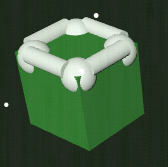
\includegraphics[scale=0.7]{./imagens/Cubo.png}
  \caption{\emph{Cubo}} \label{Fig:Cubo}
\end{minipage}%
\begin{minipage}{.5\textwidth}
  \centering
  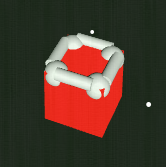
\includegraphics[scale=0.7]{./imagens/LampadaOFF.png}
  \caption{\emph{Lâmpada OFF}} \label{Fig:LampadaOFF}
\end{minipage}
\begin{minipage}{.5\textwidth}
  \centering
  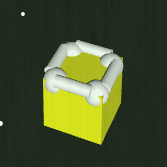
\includegraphics[scale=0.7]{./imagens/LampadaON.png}
  \caption{\emph{Lâmpada ON}} \label{Fig:LampadaON}
\end{minipage}
\begin{minipage}{.5\textwidth}
  \centering
  
\includegraphics[scale=0.4]{./imagens/proximoNivel.png}
  \caption{\emph{Próximo Nível}} \label{Fig:proximoNivel}
\end{minipage}%
\begin{minipage}{.5\textwidth}
  \centering
  
\includegraphics[scale=0.4]{./imagens/tenteDeNovo.png}
  \caption{\emph{Tente de Novo}} \label{Fig:tenteDeNovo}
\end{minipage}
\end{figure}

\begin{figure}[h!]
\centering

\includegraphics[scale=0.6]{./imagens/PaiNatal.png}
\caption{\emph{Pai Natal}} \label{Fig:Pai Natal}
\end{figure}

\begin{figure}[h!]
\centering
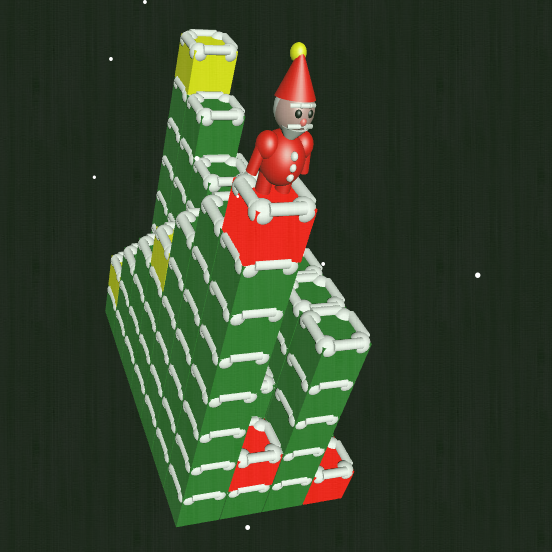
\includegraphics[scale=0.5]{./imagens/X3Dom.png}
\caption{Exemplo de um tabuleiro com várias lâmpadas e o \emph{Pai Natal}} \label{Fig:X3Dom}
\end{figure}

\paragraph{}
Criamos o ficheiro \emph{Prototipo\_X3Dom.html} com a estrutura que queriamos como resultado final.
Finalizada toda a criação, passamos à incorporação em \emph{Haskell} de todo o código \emph{html}.

Assim, dentro da pasta \emph{/src}, criámos a pasta \emph{/X3Dom} com o seguinte conteúdo:

\begin{itemize}
\item {\emph{\textbf{css}}}

O ficheiro \emph{style.css} é chamado na \emph{head} para ser usado como folha de estilo, onde definimos alguns parâmetros relativos à apresentação final da nossa página.

\item {\emph{\textbf{images}}}

Contém não mais do que a imagem que é chamada pelo \emph{Style.css}, usada como fundo da nossa página.

\item {\emph{\textbf{js}}}

De forma a proporcionar um espírito ainda mais natalício, decidimos usar um \emph{script}, escrito em \emph{JavaScript}, não tendo sido este criado por nós, mas que encontramos após alguma pesquisa, devidamente licenciado, pronto a ser utilizado.
O ficheiro \emph{snowstorm.js} é usado então para criar o efeito de queda de flocos de neve.

\emph{script DHTML Snowstorm Copyright (c) 2007, Scott Schiller. All rights reserved. Code provided under the BSD License}

\item {\emph{\textbf{shapes}}}

Contém o código \emph{X3Dom} para gerar a forma dos cubos cobertos de neve e ainda o \emph{Pai Natal}:
\end{itemize}
\paragraph{}
O restante código, tal como cores e posições, é criado em \emph{Haskell}.

\paragraph{}
Para evitar falhas de ligação às diretorias destes ficheiros, pois isso dependia do local onde iríamos abrir a nossa página final, colocamos todos estes ficheiros, à exceção das \emph{shapes}, num servidor que pudesse ser acessível online, através de um \emph{link}. Portanto, mantivemos os ficheiros na estrutura prevista, mas na verdade estes estão a ser usados a partir de um servidor privado que um dos membros possui.

\subsubsection{Implementação em \emph{Haskell}}

\paragraph{}
Começamos por criar as funções que iam gerar o tabuleiro, com as respetivas lâmpadas nas posições corretas, para tal, precisamos de algumas funções auxiliares. De seguida, colocar o \emph{robot} na sua posição inicial, algo que conseguimos sem grandes problemas. Então iniciamos a criação da animação.

\paragraph{}
Para gerar os movimentos e rotações do \emph{Pai Natal aka Robot} e o momento em que há a transição de cor dos cubos e chapéu do \emph{Pai Natal}, tivemos que gerar diferentes valores de tempo para colocar nos diferentes \emph{Key}. Esses tempos foram inicialmente definidos da seguinte forma:
\begin{itemize}
\item Salta    - 1,5 segundos
\item Anda     - 1,0 segundo
\item Esquerda - 0,5 segundos
\item Direita  - 0,5 segundos
\item Lâmpada  - 1,0 segundo
\end{itemize}
O tempo total da animação seguiu o mesmo esquema de tempos, sendo a soma de todos os comandos gerados.

\paragraph{}
Foram criadas algumas funções que permitem devolver todos estes valores correspondentes à animação do jogo. Funções essas que básicamente leem os comandos gerados/fornecidos e devolvem valores, sob forma de \emph{string}, que correspondem às diferentes posições do \emph{Pai Natal} no espaço \emph{X3dom}, bem como à sua orientação e ao tempo em que este acende as diversas lâmpadas.


\paragraph{}
Nas primeiras submissões no \emph{Mooshak} da tarefa E tivemos erros devido a algumas \emph{tags X3Dom} que não deveriam estar a ser reconhecidas na validação da tarefa. Como neste momento estamos a ler algumas formas do \emph{X3Dom} de ficheiros localizados em sub pastas da pasta \emph{src} a avaliação dá \emph{0 Presentation Error}. Decidimos ignorar essa situação, assumindo que toda a tarefa será avaliada qualitativamente pelo conteúdo do \emph{SVN}.


\subsection{Testes da tarefa E}

\paragraph{}
Os testes desta tarefa foram essencialmente criados para que o programa gerasse os comados automáticamente, também para detetarmos mais falhas na tarefa D, e alguns outros com comandos fornecidos.


\section{Ficheiro \emph{Haddock}}

\paragraph{}
Os comentários em \emph{Haddock} foram sempre feitos no final de cada tarefa, isto porque ainda tínhamos bem presente qual o objetivo de cada função e o porquê de a termos criado. A documentação \emph{haddock} contem toda a informação necessária para poder entender e trabalhar com o programa.

\section{Ficheiro \emph{runtests.sh}}

\paragraph{}
Este \emph{script} permite, através do terminal \emph{bash}, efetuar todos os testes a cada tarefa que nós criamos. Apesar de termos uma função em \emph{Haskell} para fazer o mesmo, com este \emph{script}, precisamos apenas de abrir o terminal na raiz da pasta de testes e executar o comando para correr os diversos tabuleiros de teste e guardar o \emph{output} num ficheiro \emph{*.res} que é comparado com o \emph{*.out}.

Apresenta no final "Test** OK!" se o resultado fôr igual ou "ERRO NO TESTE ** !". Se o tabuleiro não existir ignora o teste apresentando o devido \emph{output}

No caso da tarefa D, editamos o \emph{script} de forma a serem guardados no ficheiro \emph{*.out} os comandos gerados para cada teste.

Já na tarefa E, editamos novamente o \emph{script} de forma a gerar o ficheiro \emph{*.html} com a página correspondente à animação do \emph{input} fornecido.

Estes ficheiros são guardados nas pastas \emph{tarefaD\_results} e \emph{tarefaE\_results} respetivamente, localizados na raiz do projeto.


\section{Ficheiro \emph{MakeFile}}

\paragraph{}
O \emph{makefile} foi criado para que todos os elementos necessários sejam gerados com um único comando. O comando \emph{make} irá compilar todas as tarefas do enunciado, realizar os respetivos testes em cada uma delas, gerar a documentação \emph{haddock}, criar o relatório em formato \emph{PDF} e ainda eliminar os ficheiros que não são necessários.

\section{Conclusão}

\paragraph{}
Foi sem dúvida um projeto interessante que contribuiu muito para aumentar e consolidar os nossos conhecimentos no que toca à linguagem \emph{Haskell} e desenvolvermos métodos de programação. Prova disso mesmo foram as dificuldades que sentimos na fase inicial, mas que no final já ultrapassávamos com alguma facilidade.

\paragraph{}
Aprendemos também como criar um \emph{script}, neste caso para executar os testes nos programas criados por nós, e um \emph{makefile} para executar vários comandos \emph{bash} de uma vez só.
\paragraph{}
O desenvolver da tarefa também mostrou a importância de saber trabalhar com o \emph{SVN} pela sua utilidade quando estamos a trabalhar em simultâneo.
\paragraph{}
Consideramos o \emph{X3Dom} uma ferramenta bastante fácil de usar e com enorme potencial para fazer uma apresentação do trabalho que possa ser interpretada por qualquer pessoa.

\end{document}
